\chapter{Methods} \label{methods}

\section{Bicycle dynamics and stability} \label{sub:bicycle}
Bicycles are  very reliable transport vehicles and are considered the most efficient man powered form of transportation. Since the inception of the safety bicycle not much has changed with regards to the design of the two wheeled vehicle.   Bicycle design has been based on tinkering rather than equations which has resulted in little mathematical scrutiny in the available bicycle analyses. When trying to design a controller for a bicycle, a model that accurately describes its dynamics and kinematics is required but until 2007 there was no consensus on a set of equations that do that, so research on rider control for bicycles was hardly attempted. This changed when Meijaard et al.\cite{meijaard2007linearized}  developed a set of linearized equations of motion for the Whipple-Carvalho bicycle  model (fig \ref{fig:figure2}).\par
\begin{figure}[ht]
    \centering
    \includegraphics[scale=0.3]{images/figure3_1.png}
    \caption{ The Whipple-Carvalho bicycle model consists of four rigid bodies: rear wheel R, rear frame B, front frame H and front wheel F connected via hinges. The center of mass locations are expressed relative to the x - and z -coordinates shown (with origin at P and y pointing towards the reader). The other parameters shown are the steer axis tilt \ensuremath{\lambda}, wheelbase \ensuremath{w} and trail \ensuremath{c}. The model at its most expanded form is described by 25 parameters.\cite{meijaard2007linearized}}
    \label{fig:figure2}
\end{figure}
\subsection{The linearized Whipple-Carvalho bicycle model}




    For  the equations of motion to be derived several assumptions were made by Meijaard  et al.\cite{meijaard2007linearized}:

    \begin{enumerate}
        \item The rider is rigidly connected to the rear frame with the mass of the arms included in the mass.
        \item The contact between tire and ground is modelled as a non-slipping rolling point-contact, meaning
              that wheels have an ideal rotation without lateral slip.
        \item Friction between moving parts and pedaling forces is neglected. Thus, the total energy of the
              system is constant.
        \item The bicycle is moving with constant forward velocity.
    \end{enumerate}
\par
In order to understand the derived equations of motion a consideration must be made with regards to the configuration space and the velocity space of the model. The benchmark bicycle model derived is defined by 25 parameters. However, as a result of holonomic constraints (hinges and ground contacts) and non-holonomic constraints (non-slipping rolling contacts), its accessible configuration space can be reduced to 7 parameters. Coordinates \ensuremath{x_{P}} and \ensuremath{y_{P}} represent the translational position of the rear wheel point P, \ensuremath{\delta} is the steer angle, \ensuremath{\theta_{F}} and \ensuremath{\theta_{R}}  are the front and rear wheel angles respectively. Finally \ensuremath{\phi}  represents the lean angle about the x axis while \ensuremath{\psi}  represents the yaw rotation about the z axis. All this is depicted in figure \ref{fig:figure3}.
\begin{figure}[ht]
    \centering
    \captionsetup{justification=centering,margin=2cm}
    \includegraphics[scale=0.3]{images/figure3_2.png}
    \caption{Depiction of the benchmark bicycle in 3D. The cans represent a hinge between two rigid bodies. Multiple cans in series denote multiple degrees of freedom and the order of rotation.\cite{meijaard2007linearized}}
    \label{fig:figure3}
\end{figure}
\par
As it turns out some of the configuration variables do not appear in any of the equations of motion of the different parts. These so-called cyclic or ignorable coordinates are: the location of the bicycle on the plane (\ensuremath{x_{P}}, \ensuremath{y_{P}}), the heading of the bicycle \ensuremath{\psi} and the rotations (\ensuremath{\theta_{R}}, \ensuremath{\theta_{F}}) of the two wheels relative to their respective frames \cite{meijaard2007linearized}. Additionally due to a symmetry of the bicycle design and the lateral equations of motion, a  first order decoupling between forward and lateral dynamics exists \cite{meijaard2007linearized}. This means that the equations governing forward movement can be ignored when examining lateral dynamics like bicycle stabilization and vice versa. In conclusion, the three independent degrees of freedom that define the equations of motion are the  forward speed \ensuremath{\nu},  the lean angle \ensuremath{\phi} and the  steering angle \ensuremath{\delta} (figure \ref{fig:figure3}).
\subsection{The linearized equations of motion} \label{subsec:EOM}
Keeping in mind the above considerations Meijaard et al.\cite{meijaard2007linearized} managed to formulate a set of three linearized equations that each describe a degree of freedom. The first is a first order differential equation that describes the forward speed as shown in equation \ref{eq:equation1}\cite{meijaard2007linearized}.
\begin{equation}
    \left[r_{R}^{2} m_{T}+I_{R y y}+\left(\frac{r_{R}}{r_{F}}\right)^{2} I_{F y y}\right] \ddot{\theta}_{R}=T_{\theta_{R}}
    \label{eq:equation1}
\end{equation}
where \ensuremath{I}, \ensuremath{r} and \ensuremath{m} denote inertia, radius and mass respectively of the rigid body defined in the subscript. Also \ensuremath{T_{\theta_{R}}} denotes the torque applied to the rear wheel in the direction of \ensuremath{\theta_{R}}.
\par
For the two remaining degrees of freedom the lean angle(\ensuremath{\phi}) and the steer angle (\ensuremath{\delta}) they found two second-order differential equations that are coupled and are given by equation \ref{eq:equation2}\cite{meijaard2007linearized}.
\begin{equation}
    \mathbf{M} \ddot{q}+v \mathbf{C}_{1} \dot{q}+\left[g \mathbf{K}_{0}+v^{2} \mathbf{K}_{2}\right] \mathbf{q}=\mathbf{f}
    \label{eq:equation2}
\end{equation}
where \ensuremath{q} is a vector containing the roll and steer angles, \ensuremath{f} is a vector containing the roll and steer torques, \ensuremath{g} is the gravitational acceleration and \ensuremath{\mathbf{M},\;v\mathbf{C}_{1},\;g \mathbf{K}_{0}+v^{2} \mathbf{K}_{2}} are the "mass", "damping" and "stiffness" ratios in matrix form respectively.

When talking about bicycle stability and control, equation \ref{eq:equation1} is often ignored as the task of pedaling is often removed from the problem so as to focus on pure roll stabilization. For control purposes it is convenient to express the bicycle equation \ref{eq:equation2} in state-space form . The state-space representation is:
\begin{equation}
    \dot{\mathbf{x}}=\mathbf{A} \mathbf{x}+\mathbf{B} \mathbf{f}
\end{equation}
\begin{equation}
    \mathbf{y}=\mathbf{C} \mathbf{x}+\mathbf{D} \mathbf{f}
\end{equation}
where matrices \ensuremath{A,B,C,D} are defined by:
\begin{equation}
    \mathbf{A}=\begin{bmatrix}
        -\mathbf{M}^{-1}v\mathbf{C}_{1} & -\mathbf{M}^{-1}(g \mathbf{K}_{0}+v^{2}\mathbf{K}_{2}) \\
        {\mathbf{I}}                    & {\mathbf{0}}
    \end{bmatrix} , \mathbf{B}=\left[ \begin{array}{c}{\mathbf{M}^{-1}} \\ {\mathbf{0}}\end{array}\right] ,
    \mathrm{C}=\begin{bmatrix} {\mathbf{0}} & {\mathbf{I}}
    \end{bmatrix} , \mathrm{D}=[\mathbf{0}]
\end{equation}
\par
By finding the eigenvalues of matrix \ensuremath{A} one can begin asking questions regarding the stability of the system. Meijaard et al. \cite{meijaard2007linearized} found the eigenvalues for different forwards speeds and managed to determine the region in which the uncontrolled benchamark bicycle was stable. In figure \ref{fig:figure4} the four eigenvalues are plotted in a forward speed range \ensuremath{0<v<10\; ms^{-1}}. The region that is defined when the real part of the weave eigenvalue becomes negative and the capsize eigenvalue has not crossed the zero threshold yet is the stable region and corresponds to forward speeds  \ensuremath{4.3\lessapprox v \lessapprox 6\; ms^{-1}}. When designing a controller  the input signals \ensuremath{f} are tasked with influencing the poles of the characteristic polynomial and moving the system from the unstable region to a stable one.

\begin{figure}[ht]
    \centering
    \captionsetup{justification=centering,margin=2cm}

    \includegraphics[scale=0.6]{images/figure3_3.png}
    \caption{Root locus plot of the benchmark bicycle. Bold black lines indicate the real part of the eigenvalues while dotted show the imaginary part.\cite{meijaard2007linearized}}
    \label{fig:figure4}
\end{figure}

Before exploring potential control options for the bicycle model described by the above equations, it is interesting to see to what extent is the model controllable. We know that the bicycles and motorcycles are controllable in reality but how well does this model capture reality is still a question.

To determine controllability of a dynamical system the reachability matrix :

\begin{equation}
    \mathbf{Q}=\left[\mathbf{B}, \mathbf{A B}, \mathbf{A}^{2} \mathbf{B}, \cdots, \mathbf{A}^{k-1} \mathbf{B}\right]
    \end{equation}
must be full rank. When the matrix rank is equal to the number of states of the system then the system is controllable by inputs \ensuremath{f}. By taking the determinant and then solving the equation:
\begin{equation}
    det\; \mathbf{Q} = \mathbf{0}
\end{equation} 
the forward velocities that result in an uncontrollable system can be found. Schwab et al. in \cite{schwab2010controllability} isolated the control inputs and found that a Whipple like bicycle with the an extended rider model can be controlled by either lean or steer torque for the practical range of 1 to 10 \ensuremath{\frac{m}{s}}. Although some forward speeds that result in a zero determinant exist they were either extremely close to zero or part of a stable mode so they concluded that they are of no concern.




\section{The Delft steer-by-wire bicyle}

An instrumented steer-by-wire bicycle was recently developed by Delft's Bicycle Lab \cite{dialynas2019wire}. Steer-by-wire is a technology where electronic sensors and actuators are used to replace conventional mechanical systems. In this case the mechanical link between the handlebar and the fork was removed. This bicycle was the core tool used for the experimental process as it proved to be a versatile platform for rider control identification.


By removing the mechanical link an additional degree of freedom in the Whipple model  is added, the fork angle \ensuremath{\theta}. In order to simulate normal bicycle dynamics a controller is needed that will close the margin between steer angle \ensuremath{\delta} and angle \ensuremath{\theta}. This was achieved by the use of a PD-controller of the following form:


\begin{equation}
\begin{array}{l}{T_{P D H}=K_{P H}(\delta-\theta)+K_{D H}(\dot{\delta}-\dot{\theta})} \\ {T_{P D F}=K_{P F}(\delta-\theta)+K_{D F}(\dot{\delta}-\dot{\theta})}\end{array}
\end{equation}
where \ensuremath{T_{P D H}} is the torque applied by the  handlebar motor,  \ensuremath{T_{P D F}} is the torque applied by the fork motor and \ensuremath{K_{P H},K_{P F},K_{D H},K_{D F}} are the proportional and differential gains respectively. The updated input to the system is given by:
\begin{equation}
\overline{\boldsymbol{f}}=\left[ \begin{array}{c}{T_{\delta}} \\ {T_{\phi}} \\ {T_{\theta}}\end{array}\right]=\left[ \begin{array}{c}{T_{H}-T_{P D H}} \\ {T_{\phi}}  \\ {T_{P D F}}\end{array}\right]
\end{equation}
where \ensuremath{T_{H}} is the torque applied by the rider.

Using the parameters of table  \ref{tb:BIKE_parameters} the matrices of equation \ref{eq:equation2} are calculated for the steer-by-wire bicycle (see APPENDIX for full discription). Doing the root locus analysis for the updated bicycle model the stable speed region can be calculated. The stable region corresponds to speeds  \ensuremath{4.39\lessapprox v \lessapprox 6.67\; ms^{-1}} (see Fig. \ref{fig:rootlocus}).

\begin{figure}[ht]
    \centering
    \captionsetup{justification=centering,margin=2cm}

    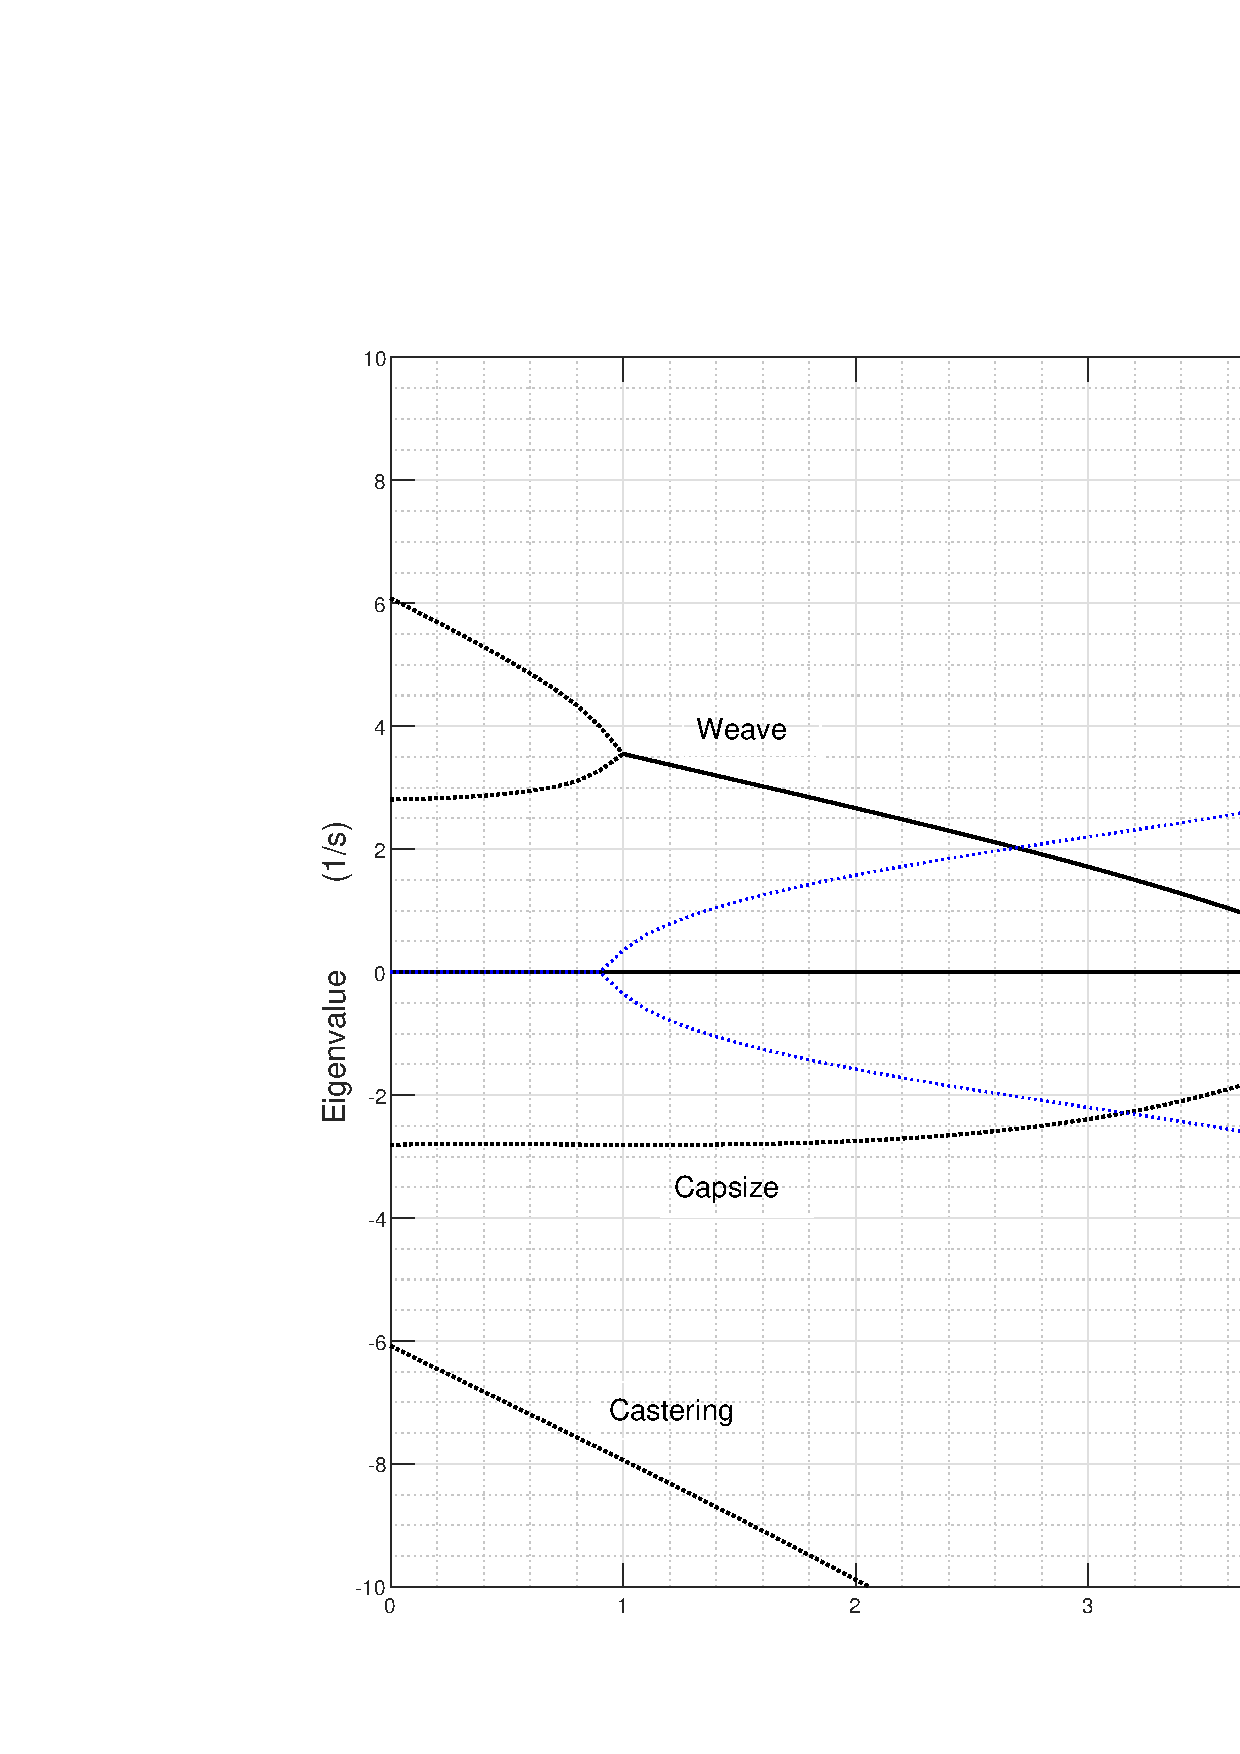
\includegraphics[scale=0.6]{images/root_locus_steerbywire.png}
    \caption{Root locus plot of the steer by wire bicycle. Dotted blue lines indicate the real part of the eigenvalues while dotted cyan show the imaginary part.}
    \label{fig:rootlocus}
\end{figure}
The bicycle has an inertia measurment unit (IMU MPU9250) that measures roll, pitch and yaw rate as well as linear accelerations. The IMU is located and oriented as shown in figure \ref{fig:IMUaxis}. It also has two rotary encoders; one in the back wheel to measure forward speed (\ensuremath{v}) and one in the pedal to measure pedal cadence. Angle encoders measure the angles \ensuremath{\delta} and \ensuremath{\theta} for the controller to function. A torque sensor was also custom made and placed in the handlebar assembly. Its purpose was to validate that the command torque to the motor is equal to the torque applied by the motor. For more regarding the torque sensor see section \ref{sec:torqueSensor}.  Finally the bike has a rear wheel motor so  a constant speed can be easily set and the pedalling task is removed from the problem. For certain necessary  signals, such as roll angle and input torque, no direct measurement from sensors were available so these signals were estimated using the methods described below.
\begin{figure}[ht]
    \centering
    \captionsetup{justification=centering,margin=2cm}

    \includegraphics[scale=0.08]{images/imu_axis_steerbywire.jpg}
    \caption{The steer-by-wire bicycle with the locations of all its sensors. The axis indicate the orientation of measurements for the IMU sensor.}
    \label{fig:IMUaxis}
\end{figure}


\begin{table}[]
    \begin{tabular}{lllll}
    \cline{1-3}
    \multicolumn{1}{l}{Parameter}                                         & \multicolumn{1}{l}{Symbol} & \multicolumn{1}{l}{Value} &  &  \\ \cline{1-3}
    wheel base                                                              & w                           & \ensuremath{1.03 m}        &  &  \\
    trail                                                                   & c                           &  \ensuremath{0.0665 m}     &  &  \\
    steer axis tilt \ensuremath{(\pi / 2-\text { head angle })  }           & \ensuremath{\lambda}        &  \ensuremath{\pi \char`\\ 10}                          &  &  \\
    rear wheel                                                              & R                           &                            &  &  \\
    radius                                                                  & \ensuremath{r_R}            &  \ensuremath{0.6858 m}     &  &  \\
    mass                                                                    & \ensuremath{m_R}            &  \ensuremath{8.5 \; kg}    &  &  \\
    mass moment of intertia                                                 &  \ensuremath{(I_{R_{xx}},I_{R_{yy}})} &  \ensuremath{(0.095625,0.19125) \;kg\;m^2}   &  &  \\
    rear body and frame assembly                                            & B                           &                            &  &  \\
    position centre of mass                                                 &  \ensuremath{\left(x_{\mathrm{B}}, z_{\mathrm{B}}\right)}              &       \ensuremath{(0.4,-0.6)}        &  &  \\
    mass                                                                    &     \ensuremath{m_B}           &  \ensuremath{95 kg}             &  &  \\
    mass moment of inertia                                                  &    \ensuremath{\left[ \begin{array}{ccc}{I_{\mathrm{Bxx}}} & {0} & {I_{\mathrm{B} x z}} \\ {0} & {I_{\mathrm{B} y y}} & {0} \\ {I_{\mathrm{B} x z}} & {0} & {I_{\mathrm{B} z z}}\end{array}\right]}            &     \ensuremath{\left[ \begin{array}{ccc}{9.2} & {0} & {2.4} \\ {0} & {11} & {0} \\ {2.4} & {0} & {2.8}\end{array}\right] \mathrm{kg\;m}^{2}}          &  &  \\
    front handlebar and fork assembly                                       & H                           &                            &  &  \\
    position centre of mass                                                 &    \ensuremath{\left(x_{\mathrm{H}}, z_{\mathrm{H}}\right)}            &   \ensuremath{(0.9,-0.66)}            &  &  \\
    mass                                                                    &     \ensuremath{m_H}           &    \ensuremath{1.5 kg}           &  &  \\
    mass moment of inertia                                                  &   \ensuremath{\left[ \begin{array}{ccc}{I_{\mathrm{H} x x}} & {0} & {I_{\mathrm{H} x z}} \\ {0} & {I_{\mathrm{Hyy}}} & {0} \\ {I_{\mathrm{Hxz}}} & {0} & {I_{\mathrm{H} z z}}\end{array}\right]}             &     \ensuremath{\left[ \begin{array}{ccc}{0.05892} & {0} & {-0.00756} \\ {0} & {0.06} & {0} \\ {-0.00756} & {0} & {0.00708}\end{array}\right] \mathrm{kg\;m}^{2}}          &  &  \\
    front wheel                                                             & F                           &                            &  &  \\
    radius                                                                  &     \ensuremath{r_F}           &    \ensuremath{0.6858 m}           &  &  \\
    mass                                                                    &     \ensuremath{m_F}           &     \ensuremath{1.84 kg}          &  &  \\
    mass moment of inertia                                                  &   \ensuremath{\left(I_{\mathrm{Fxx}}, I_{\mathrm{F} y y}\right)}             &    \ensuremath{(0.097,0.195) \mathrm{kg} \;\mathrm{m}^{2}}           &  &  \\
   battery rack                                      & b                           &                            &  &  \\
    position centre of mass                                                 &    \ensuremath{\left(x_{\mathrm{b}}, z_{\mathrm{b}}\right)}            &   \ensuremath{(0.4,-0.55)}            &  &  \\
    mass                                                                    &     \ensuremath{m_H}           &    \ensuremath{4 kg}           &  &  \\
    mass moment of inertia                                                  &   \ensuremath{\left[ \begin{array}{ccc}{I_{\mathrm{H} x x}} & {0} & {I_{\mathrm{H} x z}} \\ {0} & {I_{\mathrm{Hyy}}} & {0} \\ {I_{\mathrm{Hxz}}} & {0} & {I_{\mathrm{H} z z}}\end{array}\right]}             &     \ensuremath{\left[ \begin{array}{ccc}{0.02} & {0} & {-0.02} \\ {0} & {0.04} & {0} \\ {-0.02} & {0} & {0.02}\end{array}\right] \mathrm{kg\;m}^{2}}          &  &  \\
    
    
    \end{tabular}
    \captionsetup{justification=centering,margin=2cm}
    \caption{Whipple model parameters for the steer-by-wire bicycle shown in figure \ref{fig:IMUaxis}.}
    \label{tb:BIKE_parameters}
    \end{table}

\section{Estimation of Rider Torque}

Given  the steer rate (\ensuremath{\dot{\delta}}) and acceleration(\ensuremath{\ddot{\delta}}), moment of inertia (\ensuremath{I_H}), motor damping  (\ensuremath{b_m}) and the torque applied by the handlebar motor (\ensuremath{T_{PDH}}) the equation of motion of the upper handlebar assembly can be formed (see Fig. \ref{fig:free_handle}) and solved for the uknown rider input torque (\ensuremath{T_H}).

\begin{equation}
    T_{H}= \ddot{\delta}I_H+\dot{\delta}b_{m} -T_{PDH} 
    \label{eq:torque_rider}
\end{equation}
\begin{figure}[h]
    \centering 
    \captionsetup{justification=centering,margin=2cm}

    \captionsetup{justification=centering,margin=2cm}
    \includegraphics[scale=0.9]{images/free_handle.png}
    \caption[Short title]{Free body diagram of the upper handlebar assembly. }
    \label{fig:free_handle}
\end{figure}

\subsection{Steer rate and acceleration} \label{sec:rateAccel}
Since only the steering angle is directly measurable, a way needs to be found that produces accurate estimations of steer rate and steer acceleration. Simple numerical differencing techniques proved ineffective as noise effects were magnified resulting in completed corrupted second derivatives, even after filtering the original signal to a cutoff frequency of 10 Hz. 

To combat this problem a piecewise cubic interpolation technique using the cubic spline function was used. The principle of this method is simple. Third order polynomilas are fitted   between the datapoints. This results in a signal that is identical to the original but instead of discrete points, it is represented by the union of polynomial functions. After this point the steer rate and acceleration can be easily obtained by taking the derivatives of the polynomials. the result of the method is seen in figure \ref{fig:spline}. 
\begin{figure}[ht]
    \centering
    \captionsetup{justification=centering,margin=2cm}

    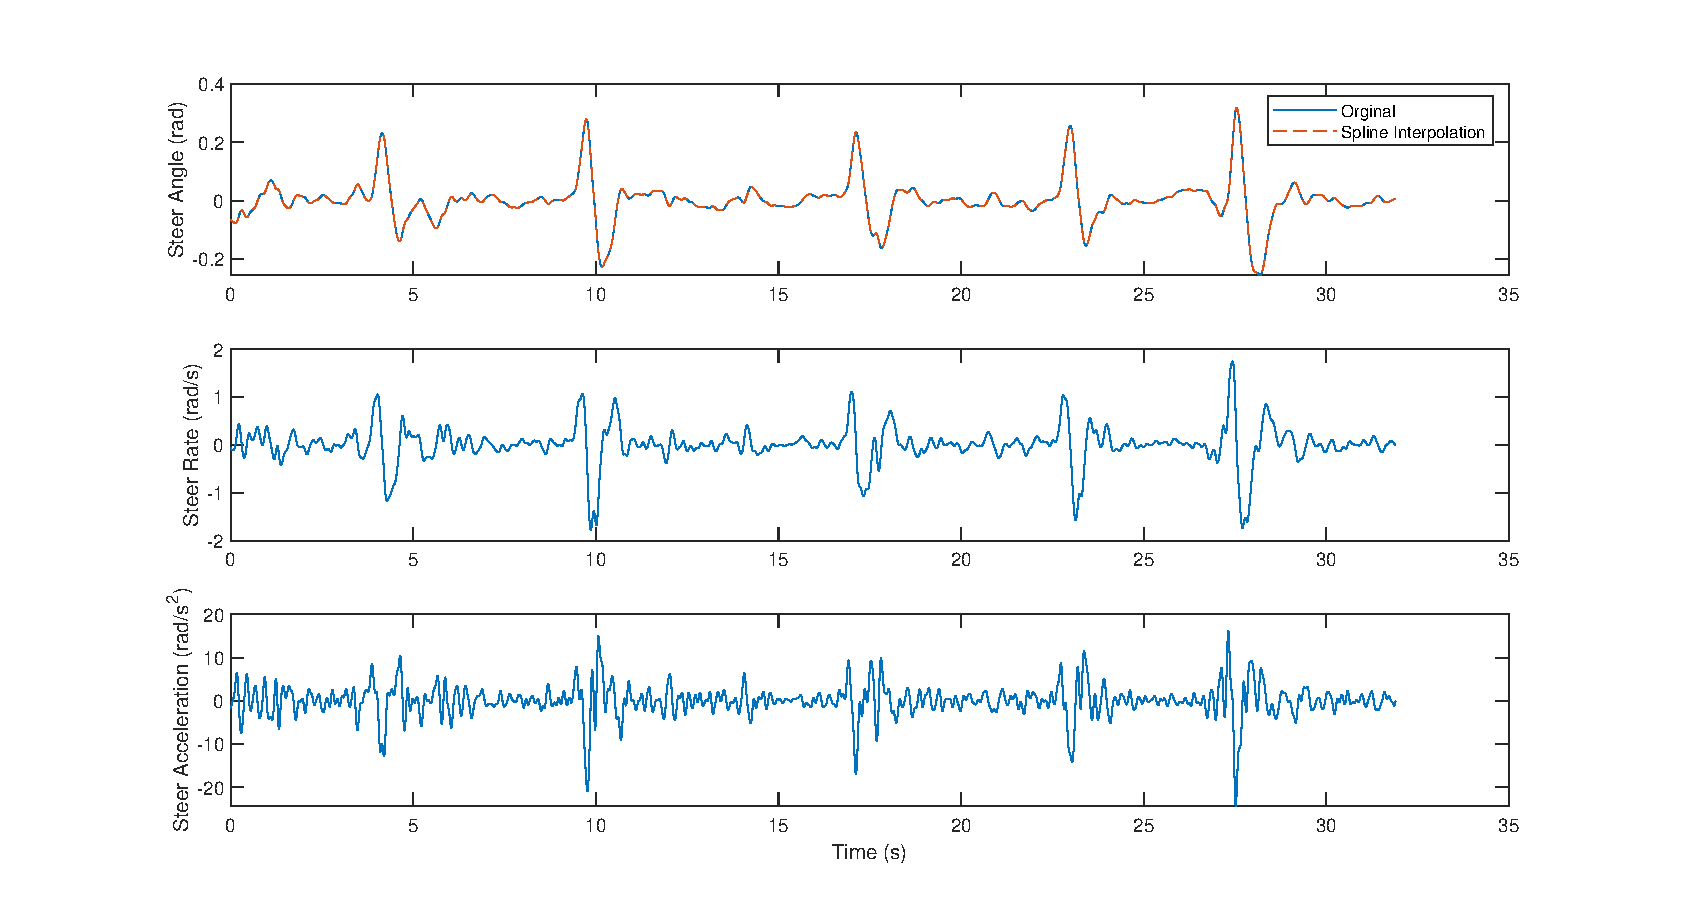
\includegraphics[scale=0.6]{images/steer_rates_spline.eps}
    \caption{Steering angle signal with its derivates produced by the piecewise cubic spline interpolation method.}
    \label{fig:spline}
\end{figure}
\subsection{Steering shaft moment of inertia and viscous friction}

In order to make estimation of applied rider torque, the damping coefficient and the inertia of the steering shaft needs to be determined. There are multiple ways to measure inertia of complex geometries. Here an estimation through a simple exprimental setup is chosen.

By connecting the steering shaft with two extension springs (see Fig.\ref{fig:figure1}) and measuring the oscillations of the steering angle \ensuremath{\delta}, a mechanical system is created where it it has to obey equation \ref{eq:1}.
\begin{equation}
    I_H\ddot{\delta}\left(t\right)+b_m\dot{\delta}\left(t\right)+2K\alpha^2\delta\left(t\right)=0
    \label{eq:1}
\end{equation}
where \ensuremath{K} the spring elastic constant and \ensuremath{\alpha} the moment arm shown in figure \ref{fig:figure1}. 
\begin{figure}[h]
\centering
\captionsetup{justification=centering,margin=2cm}
\includegraphics[scale=0.9]{images/figure1.png}
	\caption[Short title]{Spring-handlebar assembly  where \ensuremath{\alpha}  is the moment arm.}
\label{fig:figure1}
\end{figure}

 The springs ( \ensuremath{K=555 N/m} and slack length of \ensuremath{ 0.03m}) are attached to the handlebar and the system is perturbed. The measured steering angle signal from one of the perturbation tests is shown in figure \ref{fig:figure3}.The steering rate and acceleration signals are derived by the methods descirbed in section \ref{sec:rateAccel}. Equation \ref{eq:1} is then applied to all discrete time steps and so the system of equations \ref{eq:leastSquaresTORQUE} is created.
 \begin{equation}
     \begin{bmatrix}
         \ddot{\delta}_1 & \dot{\delta}_1   \\ \ddot{\delta}_2 & \dot{\delta}_2 \\ \vdots & \vdots \\ \ddot{\delta}_N & \dot{\delta}_N 
     \end{bmatrix} \begin{bmatrix}
         I_H \\ b_m
     \end{bmatrix} = -2K\alpha^2 \begin{bmatrix}
         \delta_1 \\ \vdots \\ \delta_N
     \end{bmatrix}
     \label{eq:leastSquaresTORQUE}
 \end{equation}
where \ensuremath{N} the length of the recorded signal.

Since equation \ref{eq:leastSquaresTORQUE} is linear in the parameters, the solution of the regression problem can be approximated by the use of the least squares method.
\begin{equation}
 \begin{bmatrix}
    I_H \\ b_m
\end{bmatrix} = -2K\alpha^2 \left(      \begin{bmatrix}
    \ddot{\delta}_1 & \dot{\delta}_1   \\ \ddot{\delta}_2 & \dot{\delta}_2 \\ \vdots & \vdots \\ \ddot{\delta}_N & \dot{\delta}_N 
\end{bmatrix} ^{T}       \begin{bmatrix}
    \ddot{\delta}_1 & \dot{\delta}_1   \\ \ddot{\delta}_2 & \dot{\delta}_2 \\ \vdots & \vdots \\ \ddot{\delta}_N & \dot{\delta}_N 
\end{bmatrix} \right)^{-1}      \begin{bmatrix}
    \ddot{\delta}_1 & \dot{\delta}_1   \\ \ddot{\delta}_2 & \dot{\delta}_2 \\ \vdots & \vdots \\ \ddot{\delta}_N & \dot{\delta}_N 
\end{bmatrix} ^{T}  \begin{bmatrix}
    \delta_1 \\ \ldots \\ \delta_N
\end{bmatrix}
\label{eq:leastSOLUTION}
\end{equation}
The system is perturbed 15 times so 15 sets of inertia and damping ratios are computed. The mean of the these was taken and  resulted in  \ensuremath{I_H = \mathbf{0.0960 \;kg\; m^2}} and   \ensuremath{b_m = \mathbf{0.2663\; N\; s^{-1}}}



\begin{figure}[h]
\centering
\captionsetup{justification=centering,margin=2cm}

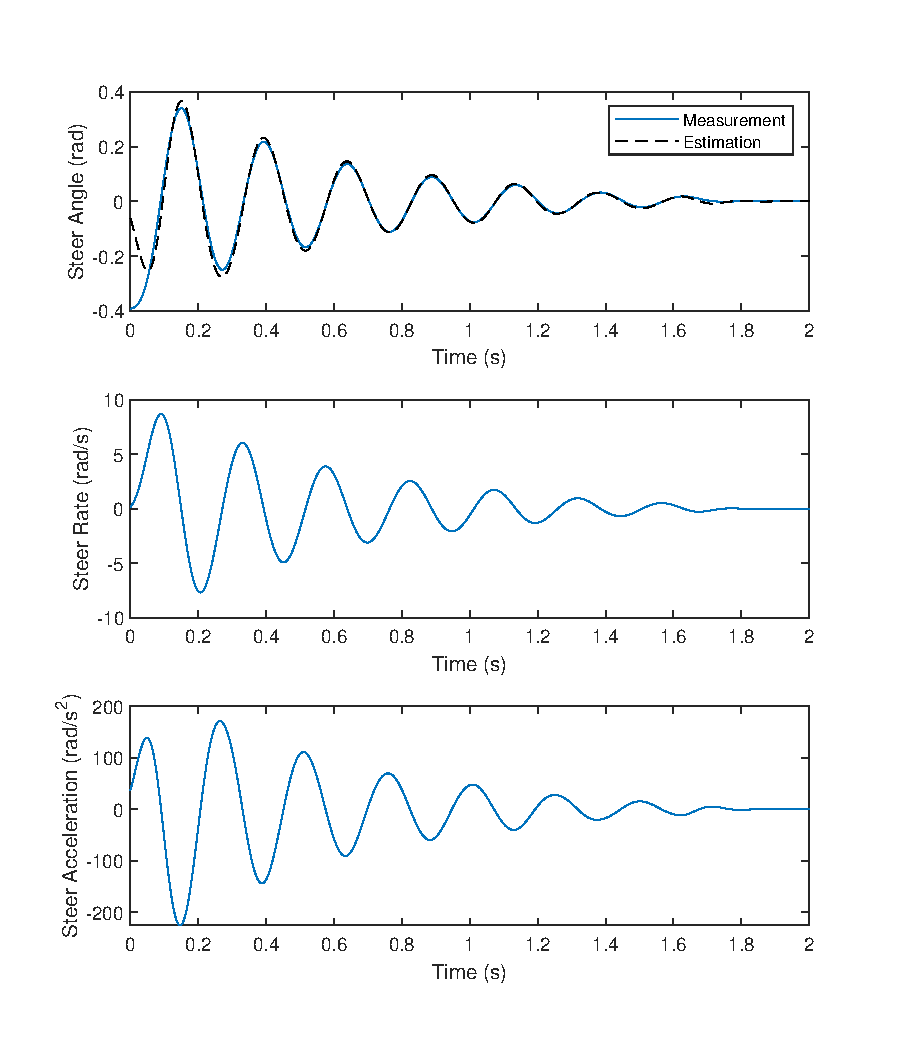
\includegraphics[scale=0.8]{images/figure3.eps}
	\caption[Short title]{Result of the first of fifteen oscillations. Blue lines indicate the  measured signals while the black dotted line is the output of the model given the values of inertia and damping estimated with the least squares method.}
\label{fig:figure3}
\end{figure}


% The damping coefficient is  \ensuremath{b=\mathbf{0.5845} \mathbit{Nms} }
\newpage
\subsection{Motor Torque Input Validation} \label{sec:torqueSensor}

\subsubsection{Design of torque sensor}
In order to validate that the torque exerted by the handlebar motor results in equivalent input rider torque  a torque sensor is designed and attached to the steering shaft. The most common torque sensor measurement principle uses bonded strain gauge technology, where the strain gauges are bonded to a suitably designed shaft.

In the torsion of a cylindrical shaft the strain is measured by the angle of twist or angular deflection. Unfortunately stain gauges can only detect compressive and tensile strain. The strain gauges are placed with such an orientation that the shearing stress is replaced by its equivalent principal stresses. The angle and the magnitude of the principal stresses are calculated by the use of the Mohr Circle. In this case the principal tension and compressive stresses are of the same magnitude as the shearing stress and are active at an angle of 45 degrees since it is  considered that no external compressive or tension force is present. 

In order to design a proper cylindrical shaft for the torque sensor the diameter of the shaft is chosen such that the strain measured in the strain gauges is within the detectable range (\ensuremath{\epsilon_{min}=10^{-5}} , \ensuremath{\epsilon_{max}=6\cdot10^{-4}}). For this application,  a hollow cylindrical shaft made of aluminum( \ensuremath{AL7075-O})is used so the unknowns are the inner and outer diameters. The strain is given in relation to the stress by Hooke’s law for isotropic materials by equation (\ref{eq:4}). The shearing stress is in turn given by equation (\ref{eq:5}). 


\begin{equation}
\epsilon=\frac{\sigma\cdot (1+\nu)}{E}
\label{eq:4}
\end{equation}

where \ensuremath{\nu} the Poisson's ratio and E the Young's Modulus (\ensuremath{Pa})
\begin{equation}
\tau=\frac{T\cdot r}{J}
\label{eq:5}
\end{equation}
where \ensuremath{J} is the polar moment of inertia (\ensuremath{m^4}), \ensuremath{r} the distance from center to stressed surface in the given position (\ensuremath{mm}), \ensuremath{T} the twisting moment (\ensuremath{Nm}).
 The polar moment of inertia of a circular hollow shaft can be expressed as
\begin{equation}
J = \frac{\pi \cdot (D^4 - d^4)} {32}                          
\label{eq:6}
\end{equation}
where \ensuremath{d} is shaft inside diameter (\ensuremath{mm}) and \ensuremath{D} is the shaft outside diameter (\ensuremath{mm}).

By inputing the above equations into a MATLAB script figure \ref{fig:figure4} was produced. The figure was created for a fixed inner diameter of \ensuremath{12 mm}, due to limitations in the machining process. It is evident that the lower the width of the shaft the higher detection of the low level torques. For this reason a width of 2 mm was chosen. This still means that  torques below \ensuremath{0.2 Nm } are not detectable. However the purpose of the torque sensor is not to provide acurate online measurements but to validate the input torques from the handlebar motor. The design of the resulting part is shown in \ref{fig:figure5}. 


\begin{figure}[h]
\centering
\captionsetup{justification=centering,margin=2cm}
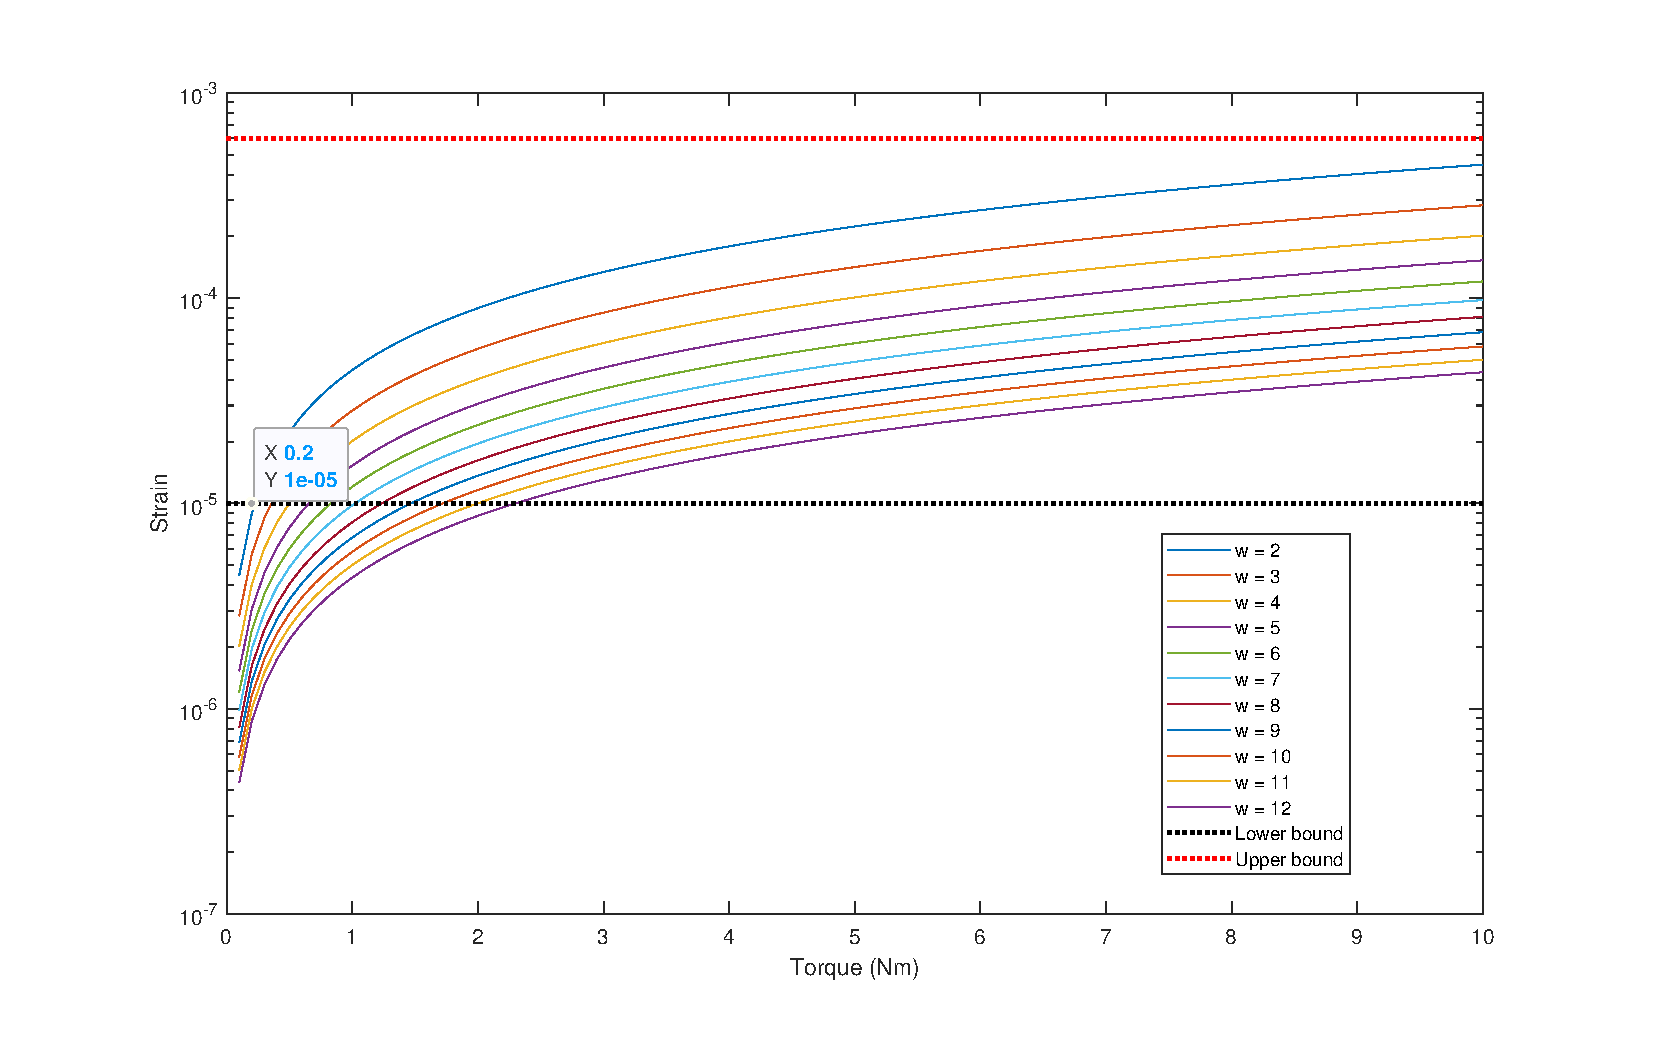
\includegraphics[scale=0.5]{images/figure4.eps}
	\caption[Short title]{Principal tensile strain in the 45 degree angle for various shaft widths (w).}
\label{fig:figure4}
\end{figure}


\begin{figure}[h]
\centering
\captionsetup{justification=centering,margin=2cm}

\includegraphics[scale=0.4]{images/sensor_schematic.png}
	\caption[Short title]{Schematic of the hollow shaft.}
\label{fig:figure5}
\end{figure}
\newpage
Because it is not an ideal hollow cylinder , the shearing stress  calculated analytically from the above equations needs to be validated. A static load simulation in SolidWorks is done to see how much different  is the shearing stress on the external surface. As it turns out the simulation showed a shearing stress similar to the one calculated by the equations. In \ref{fig:figure6} the simulation results for a loading of \ensuremath{10 Nm} is shown. For comparison the resulting shearing stress calculated analytically  is \ensuremath{10.0874\cdot 10^6 N/m^2 }. For proper measurements of  strain  the gauge  placement should gravitate towards the middle to avoid the spikes of shearing stress near the intersections between the main shaft and the cylindrical heads (see fig. \ref{fig:figure6})

\begin{figure}[h]
\centering
\captionsetup{justification=centering,margin=2cm}

\includegraphics[scale=0.6]{images/sensor_shear_SW.png}
	\caption[Short title]{Shearing stress for \ensuremath{10 Nm} loading in the axial direction.}
\label{fig:figure6}
\end{figure}

\subsubsection{Results}
In order to validate that the commanded torque in the handlebar motor is the same as the one actually applied in the handlebar, a trial identification run was conducted to simulate steer torque levels of the experiments. The signal of the input motor torque is compared with the output of the custom made torque sensor. The results are shown in figure \ref{fig:figure7}. The mismatch of the two signals for values lower than \ensuremath{0.5 Nm} is attributed to the fact that the sensor's strain gauges cannot accurately measure the strain in the material to produce realiable ouput as determined analytically beforehand. Also during the measurements a slight bias of the sensor was noted when  \ensuremath{0<\delta<\pi \char`\\
2}. Despite the aforementioned , the resulting Variance Accounted For (VAF) was equal to \ensuremath{90.77 \%} and was deemed that the motor command torque  is indeed what is beeing applied in the steering shaft so in all subsequent calculation it was taken as ground truth.

\begin{figure}[h]
    \centering
    \captionsetup{justification=centering,margin=2cm}

    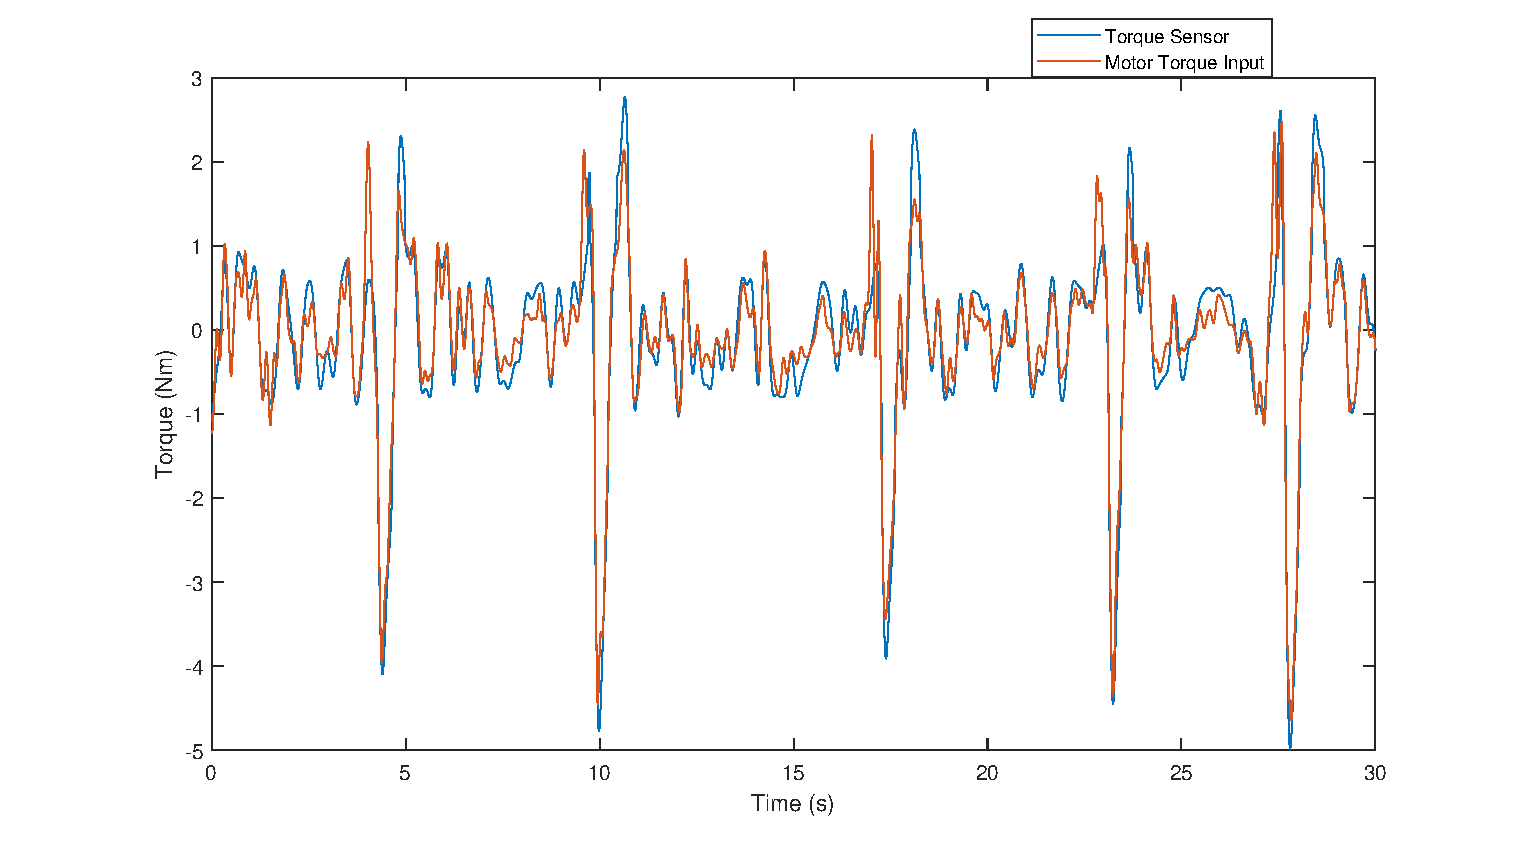
\includegraphics[scale=0.5]{images/results_torque_sensor.eps}
        \caption[Short title]{Measurement of torque sensor compared to the commanded torque of the handlebar motor.}
    \label{fig:figure7}
\end{figure}

\section{Roll Angle Estimation}
The need for reliable and accurate measurements of roll angle are paramount. Unfortunately, the steer-by-wire bike does not have sensor that can directly produce measurements of roll angle. For this reason an inderict approach is used that was developed by \citet{sanjurjo2018roll}. The method produces satisfactory roll angle estimations using only the angular rates measured by an IMU sensor.

Kalman filters are often used as state estimators when multiple measurument sources need to be combined into a single more reliable one. Often the output of a model is combined with absolute measurements and an estimation of the state is made by dynamically weighting the two sources of information. In this case a simple plant model is created which has the roll rate from the IMU as input and  produces the roll angle of the next time step given the previous one. In order to account for biases in the angular rate sensor an extra state \ensuremath{b_x} is added to the model. The complete formulation is given by :
\begin{equation}
\left[ \begin{array}{c}{\hat{\phi}} \\ {\hat{b}_{x}}\end{array}\right]_{k}^{-}=\left[ \begin{array}{cc}{1} & {-d t} \\ {0} & {1}\end{array}\right] \left[ \begin{array}{c}{\hat{\phi}} \\ {\hat{b}_{x}}\end{array}\right]_{k-1}^{+}+\left[ \begin{array}{c}{d t} \\ {0}\end{array}\right] \omega_{x, k-1}^{B}
\end{equation}
where \ensuremath{\omega_{x}^{B}} is the angular rate IMU measurement in the x direction (see Fig.\ref{fig:IMUaxis}), \ensuremath{k} indicates the current time step and \ensuremath{dt} is the time step. 


In the correction stage of the Kalman filter absolute measurements of the roll angle are needed, but such measurements are not available. For this reason equations \ref{eq:rolangle1} and \ref{eq:rolangle2} are used as pseudo absolute measurements. Sanjuro et al. explain that equation \ref{eq:rolangle1} is more reliable for roll angles close to zero and equation \ref{eq:rolangle2} is more reliable for larger roll angles, for this reason  a weighted sum of the two methods is employed \ref{eq:rolangle3} that follows the weighting function \ref{eq:rolangle4} .
\begin{align}
      \phi_{d}=\arctan \left(\frac{\omega_{z}^{B} v}{g}\right) \label{eq:rolangle1}
    \\
      \phi_{\omega}=\arctan \left(\frac{\omega_{y}^{B}}{\omega_{z}^{B}}\right)\label{eq:rolangle2}
      \\
      \phi_{m}=W \phi_{d}+(1-W) \phi_{\omega} \label{eq:rolangle3} 
      \\
      W=\exp \left(-\frac{\hat{\phi}^{2}}{\overline{\phi}^{2}}\right)
  \label{eq:rolangle4}
\end{align}


where \ensuremath{\omega_{y}^{B},\omega_{z}^{B}} are the angular rate IMU measurements in the y and z direction respectively (see Fig.\ref{fig:IMUaxis}), \ensuremath{W } is the weighting fucntion  \ensuremath{\hat{\phi}} is the last available estimation of roll and \ensuremath{\overline{\phi}^2} is a constant that can be used to adjust the weighting function. In \cite{sanjurjo2018roll} Sanjuro et al. used  \ensuremath{\overline{\phi}^2=0.05}.

 The method was used in a trial rider identification run to test if it can estimate the ranges of roll angle sway present during the experiments. The output is seen in  \cref{fig:rollangleobserverplot}. From the result it is evident that the pseudo-absolute measurements are  quite noisy. For this reason emphasis was focused on the model by tuning the initial values of covariance of the model state estimation to be much lower than that of the measurements.

 \begin{figure}[h]
    \centering
    \captionsetup{justification=centering,margin=2cm}
    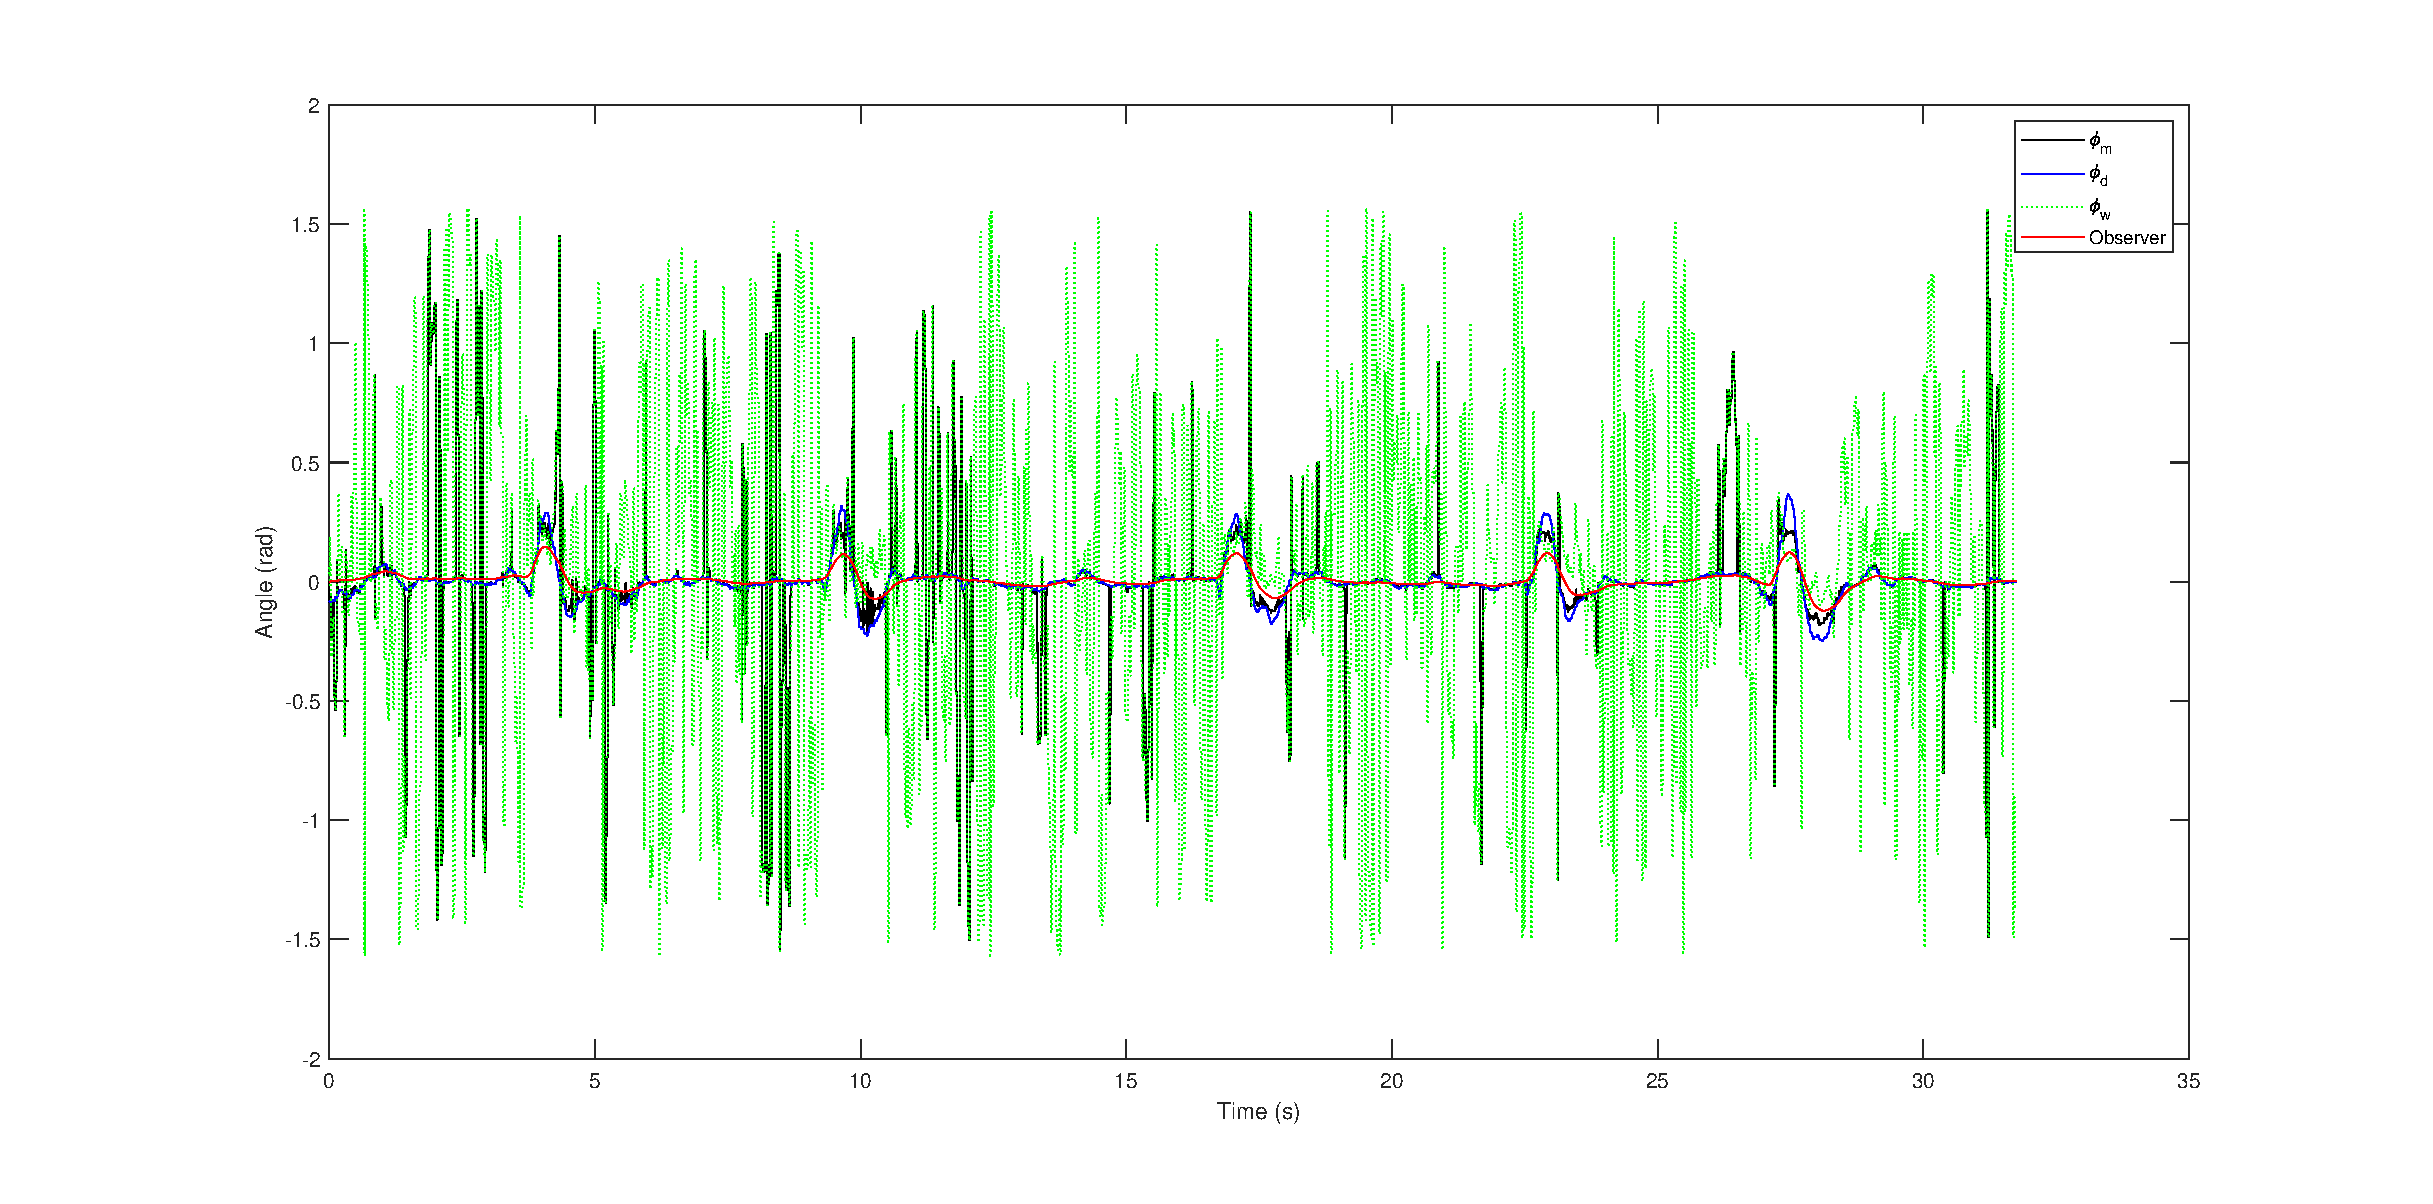
\includegraphics[scale=0.4]{images/rollangle_plot.eps}
        \caption[Short title]{Roll angle estimation output from the trial run. The red line indicates the final ouput of the kalman filter.}
    \label{fig:rollangleobserverplot}
\end{figure}
% sanjurjo2018roll